%任何有关社会保险的选题均可,期末论文具体题目请自拟
%论文请用A4纸,字体宋体、正文字号五号,论文正文部分不超过15页。
\documentclass[a4paper,12pt]{ctexart}
\usepackage[style=gb7714-2015ay]{biblatex}
\usepackage{graphicx}
\usepackage{amsmath}
\usepackage{amssymb}
\usepackage{float}
\usepackage[hidelinks]{hyperref}
\providecommand{\keywords}[1]{\\\textbf{\textit{关键词:}}#1}
\addbibresource{reference.bib}
\title{个人养老金:让第三支柱真正成为支柱}
\author{董晨阳}
\date{\today}
\begin{document}
\maketitle
\begin{abstract}
在这里写摘要。
\keywords{关键词1,关键词2}
\end{abstract}
\clearpage
\section*{个人养老金的时代背景}
2022年4月,国务院办公厅发布《关于推动个人养老金发展的意见》,标志着中国个人养老金已经取得制度层面的突破。2022年6月,人力资源社会保障部、财政部、国家税务总局、银保监会、证监会联合印发《关于推动个人养老金发展的意见》宣传提纲,加速推进政策落地。11月,《个人养老金实施办法》、《个人养老金投资公开募集证券投资基金业务管理暂行规定》、《商业银行和理财公司个人养老金业务管理暂行办法(征求意见稿)》、《关于个人养老金有关个人所得税政策的公告》等政策落地,明确了个人养老金参与流程、税收优惠等细节,完善了个人养老金相关产品规定。

我国以基本养老保险为基础、企业年金和职业年金为补充、个人储蓄性养老保险和商业养老保险相衔接的“三支柱”体系,对应当前国际养老体系的一般基准。个人养老金属于第三支柱,与前两支柱的不同在于:第一支柱基本养老保险由国家强制实施,个人养老金由个人自愿参加;第二支柱企业年金、职业年金由用人单位及其职工建立、共同缴费,个人养老金由个人缴费。从三支柱的规模占比来看,第一支柱占主导。截至2021年底,我国第一支柱基本养老金总规模约6.4万亿元,已覆盖超过10.3亿人;第二支柱约为4.5万亿元,参加职工超7000万人;第三支柱刚刚起步,我国商业养老保险责任准备金积累规模0.6万亿元。三大支柱总规模约11万亿元,一、二、三支柱分别占比67\%,29\%和4\%,合计约占GDP的13.4\%。

个人养老制度推进的背景因素包括以下几个方面:
\begin{enumerate}
    \item 中国养老体系发展较快但仍相对薄弱,三支柱总量规模仍显不足。如前文所述,当前三大支柱合计规模11万亿元,占GDP的比例为13\%,略低于OECD平均水平(2020年为14\%),与部分发达国家相比更是有较大差距,2020年加拿大、英国等发达国家的养老金储备占GDP比重普遍超过100\%,,美国三支柱规模占GDP比例为171\%。虽然我国的财政实力(增加财政用于社保的支出)及保障储备(划转国资充实社保)都可以作为居民养老的潜在补充,但是这些并不能替代三支柱体系。
    \begin{figure}[H]
        \centering
        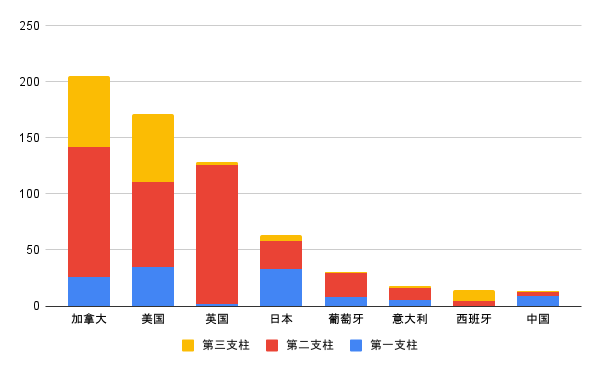
\includegraphics[width=\linewidth]{img/三支柱规模占GDP比重.png}
        \caption{2020年三支柱规模占GDP比重}
        \label{fig:GDPin2020}
    \end{figure}
    \item 三支柱规模并不均衡,目前仍以第一支柱为主。近年我国对于第二、三支柱发展的重视程度明显提升,结合前文所述,截止2021年底,三个支柱的规模占比为67\%:29\%:4\%,相较十年前第一支柱规模占比接近90\%的情况已经有明显改观。但是相较其他主要国家的情况来看,目前我国的三支柱占比仍不均衡,第一支柱的占比依然偏高。对比美国来看,美国当前三大支柱养老金的总规模分别为8.0万亿美元、14.8万亿美元和16.5万亿美元,占比为20\%:38\%:42\%,也由此可见美国的雇主养老金计划(第二支柱)和个人养老金计划(第三支柱)在美国整个养老金体系的重要性。未来第一支柱的扩大可能受制于缴费率和人口老龄化问题。中国第一支柱城镇职工基本养老保险合计缴费率为24\%,其中企业缴纳16\%,个人缴纳8\%,相对比美国第一支柱的有效缴费率仅为10.6\%,同属亚洲国家的日本和韩国分别为8.3\%和9\%。这使得我国企业的税费负担相对较重。与此同时,伴随我国人口老龄化加深,未来养老负担明显加重。目前老年赡养率为18.5\%,低于OECD平均水平(30.4\%),2050年中国老年赡养率可能上升至接近50\%,2080年进一步上升至60\%。在缴费率难以进一步提升,养老支出在老龄化趋势下可能增加的背景下,第一支柱的规模较难扩大,甚至面临财务持续性问题。2014年城镇职保的征缴收入开始低于基金支出。为维持基金正常运营,各级政府财政补贴力度逐年提高。即便计入政府财政补贴,2020年城镇职保仍出现近7000亿元的收支缺口,基金累计结存首次出现下降。城乡居保只有个人账户来自缴费,统筹账户资金原本就由国家财政承担,因此自设立之初征缴收入就一直低于基金支出。因此,在第一支柱扩容可能受限的背景下,我国第二、三支柱(补充养老保险)发展对于我国养老金体系保障能力的提升具有重要意义。
    \item 除了第一支柱外,发展个人养老制度也客观上有助于对冲其他养老方式面临的困境。例如结合世界银行对“第四支柱”的表述,房屋资产用于个人养老也是此前中国试点的一个方向。2014年6月,《关于开展老年人住房反向抵押养老保险试点的指导意见》出台,在北京、上海、广州、武汉开展住房反向抵押养老保险试点,2018年进一步将试点范围扩大至全国,但效果有限,呈现“供需双冷”局面。事实上,许多发达国家的住房反向抵押市场同样发展受阻。例如澳大利亚65岁以上老人中选择住房反向抵押的数量占比仅为1-2\%,价值占比0.4\%\citep{productivity2015australia};美国约有12-14\%的老年人符合住房反向抵押的参与条件,但参与率低于2\%\citep{warshawsky2017retire}。而且“以房养老”可能会增加居民部门杠杆率,有降低金融稳定性的潜在风险;投资房产相当于对养老储备征收“累退税”,高收入阶层房屋投资需求高,可以有效转化为养老储备;而低收入阶层以刚性使用需求为主,较难分享房屋价值升值的福利。
\end{enumerate}


\section*{文献综述}

\section*{个人养老金现状}
\subsection*{当前政策扶持}

\subsection*{产品现状}

\section*{个人养老金现国际经验}

\section*{个人养老金现前景展望}

\section*{结论}

\nocite{*}
\printbibliography[heading=bibliography,title=参考文献]
\end{document}
